\documentclass[11pt, a4paper]{article}

\usepackage[T1]{fontenc}
\usepackage[utf8]{inputenc}
\usepackage[margin=2.5cm]{geometry}
\usepackage{graphicx}
\usepackage{subcaption}
\usepackage{booktabs}
\usepackage{amsmath}
\usepackage{hyperref}
\usepackage{parskip}

\hypersetup{colorlinks=true, linkcolor=blue, urlcolor=blue}

\title{\textbf{Convergence Study: 300$\times$300 Lid-Driven Cavity}\\
       \large Worksheet 3 --- MPI Parallelisation}
\author{}
\date{}

\begin{document}

\maketitle

% ─────────────────────────────────────────────────────────────────────────────
\section{Setup}
% ─────────────────────────────────────────────────────────────────────────────

The simulation parameters are taken directly from the worksheet specification
for the lid-driven cavity benchmark on a $300\times300$ grid. The worksheet
requires the MPI configurations (serial), $(1\times1)$, $(2\times2)$, and
$(1\times4)$. To allow a more comprehensive comparison --- in particular to
examine whether the decomposition shape matters independently of the process
count --- additional configurations $(4\times1)$, $(3\times2)$, $(2\times3)$,
and $(3\times3)$ were included. All configurations use identical parameters;
only the domain decomposition ($\mathtt{iproc} \times \mathtt{jproc}$) differs
between runs.

All simulations were conducted on an \textbf{Apple M4} machine with
\textbf{16\,GB RAM}. The M4 processor features a heterogeneous core
architecture: \textbf{4 Performance cores} (P-cores) and \textbf{6 Efficiency
cores} (E-cores), totalling 10 physical cores. This distinction is critical for
interpreting the parallel results. P-cores operate at significantly higher clock
speeds and are optimised for compute-intensive workloads, while E-cores are
designed for low-power background tasks and deliver substantially lower
floating-point throughput. For MPI parallelisation, this asymmetry has a direct
consequence: since all ranks must synchronise at every communication step (halo
exchange and global reduction), the entire simulation is \textbf{bottlenecked by
the slowest participating process}. If any rank is scheduled on an E-core, every
other rank must wait for it at each synchronisation point, regardless of how fast
they completed their local computation.

Based on this architecture, the \textbf{theoretical maximum number of MPI
processes that can run without performance degradation is~4} --- matching the
number of P-cores exactly. Configurations using up to 4 ranks can be scheduled
entirely on P-cores, yielding consistent and efficient parallel execution.
Configurations with 5 or more processes inevitably spill onto E-cores,
introducing load imbalance that grows with the process count. This is confirmed
by the measured results: the 4-rank configurations achieve 80--81\% parallel
efficiency, the 6-rank configurations drop to 63--64\%, and the 9-rank
$(3\times3)$ configuration --- where 5 of 9 processes are forced onto E-cores
--- collapses to just 16\% efficiency despite using the most processes.

% ─────────────────────────────────────────────────────────────────────────────
\section{SOR Iterations per Timestep}
% ─────────────────────────────────────────────────────────────────────────────

All setups completed exactly \textbf{360\,015 timesteps} with an adaptive
timestep of $\Delta t \approx 1.39\times10^{-4}$. Three distinct phases are
observed in all configurations (see Figure~\ref{fig:sor_all}):

\textbf{Phase~1 --- Startup (steps 1--5000):} The solver hits
$\mathtt{itermax} = 100$ every timestep. The pressure field is being built up
from rest. The adaptive timestepping immediately corrects $\Delta t$ to
$\approx1.39\times10^{-4}$ from step~2 onwards.

\textbf{Phase~2 --- Rapid drop (steps 5000--15\,000):} As the primary vortex
forms, the pressure field becomes physically consistent and the SOR converges
well within the iteration limit. Iterations drop sharply from 100 to
approximately~5.

\textbf{Phase~3 --- Quasi-steady state (steps 15\,000--360\,015):} All setups
maintain a stable median of~5 SOR iterations per timestep with occasional spikes
of 6--8. Only 1.39--1.44\% of all timesteps reach the iteration limit.

Crucially, the SOR iteration counts are \textbf{numerically identical across all
MPI configurations} (mean: 8.04--8.13, median: 5 for all setups). This confirms
that the domain decomposition does not affect the numerical behaviour of the
pressure solver --- the global residual yields the same stopping criterion
regardless of how the domain is partitioned.

% 2x2 figure grid
\begin{figure}[htbp]
    \centering
    \begin{subfigure}[t]{0.48\textwidth}
        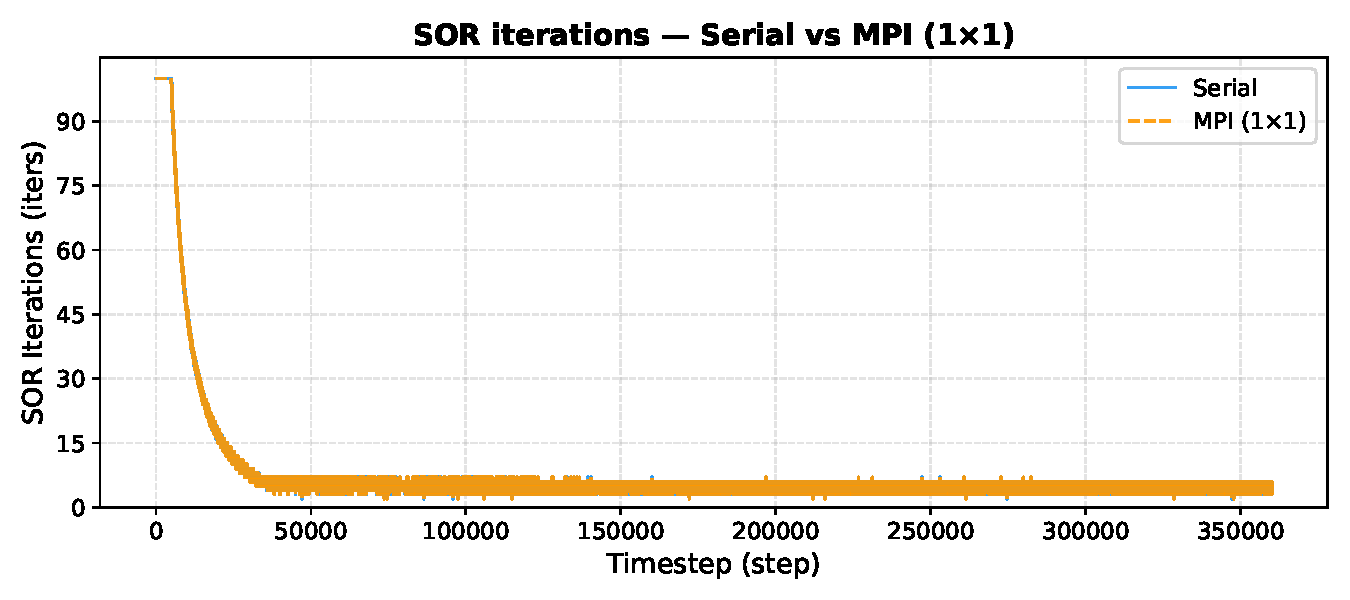
\includegraphics[width=\textwidth]{plot_sor_serial_vs_11.pdf}
        \caption{Serial vs.\ MPI $(1\times1)$}
        \label{fig:sor_serial}
    \end{subfigure}
    \hfill
    \begin{subfigure}[t]{0.48\textwidth}
        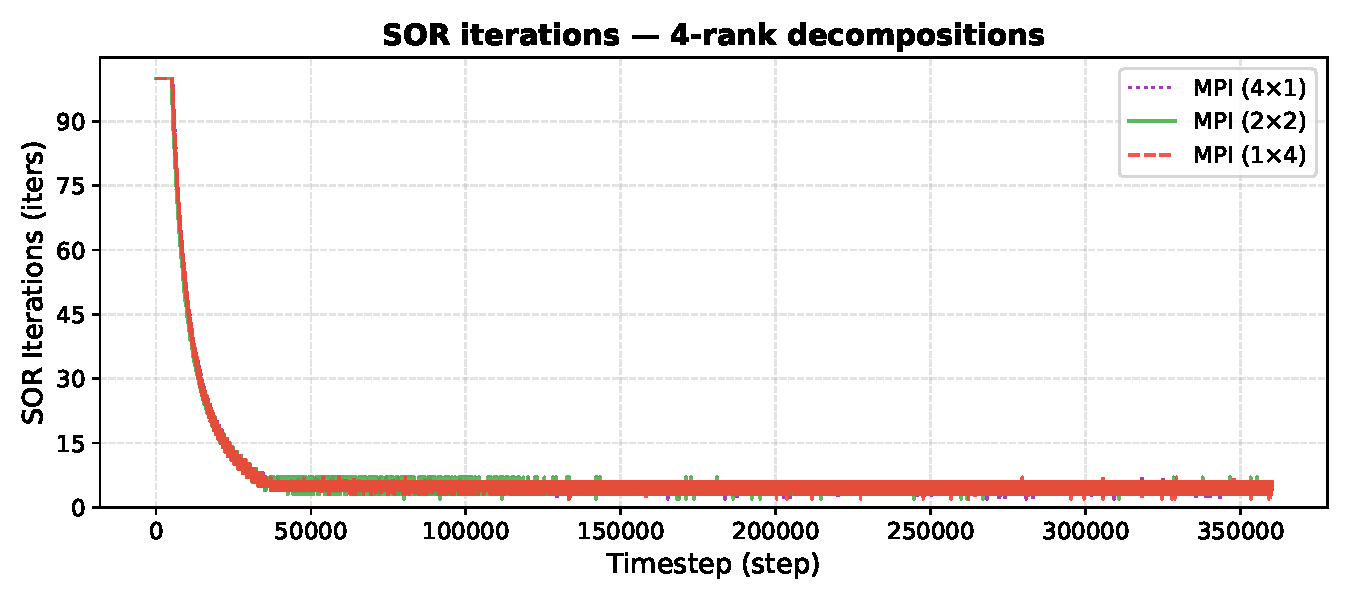
\includegraphics[width=\textwidth]{plot_sor_4ranks.pdf}
        \caption{4-rank decompositions: $(2\times2)$, $(1\times4)$, $(4\times1)$}
        \label{fig:sor_4ranks}
    \end{subfigure}

    \vspace{0.8em}

    \begin{subfigure}[t]{0.48\textwidth}
        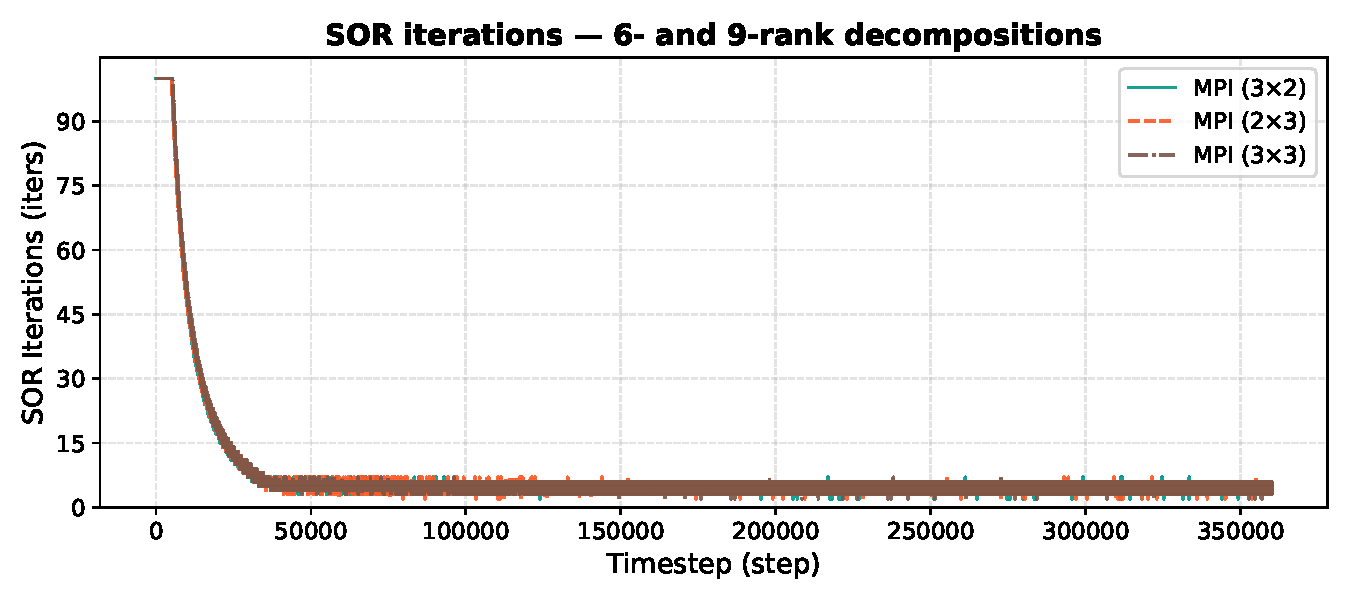
\includegraphics[width=\textwidth]{plot_sor_6_9ranks.pdf}
        \caption{6- and 9-rank decompositions}
        \label{fig:sor_69ranks}
    \end{subfigure}
    \hfill
    \begin{subfigure}[t]{0.48\textwidth}
        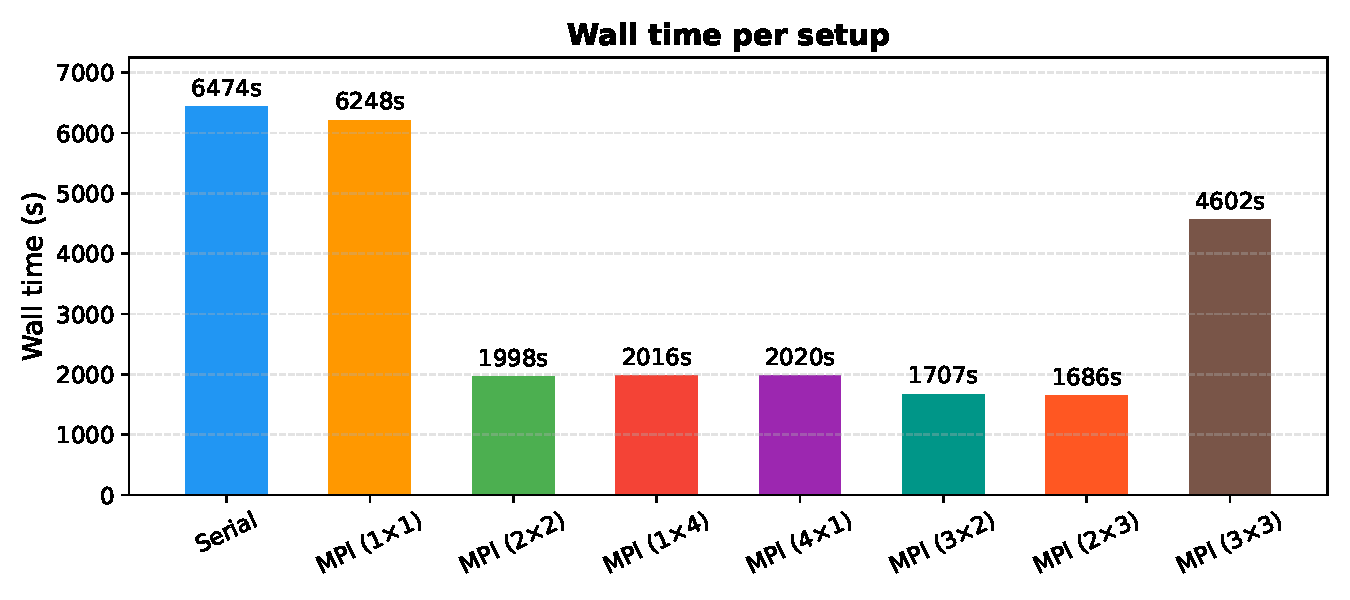
\includegraphics[width=\textwidth]{plot_runtime.pdf}
        \caption{Wall time and speedup}
        \label{fig:runtime}
    \end{subfigure}

    \caption{SOR iterations per timestep for all MPI configurations (top left,
             top right, bottom left) and runtime comparison (bottom right).
             All SOR plots show identical convergence behaviour regardless of
             decomposition.}
    \label{fig:sor_all}
\end{figure}

% ─────────────────────────────────────────────────────────────────────────────
\section{Runtime and Speedup}
% ─────────────────────────────────────────────────────────────────────────────

\begin{table}[htbp]
    \centering
    \caption{Wall time, speedup, and parallel efficiency for all configurations.
             Speedup is computed relative to the serial run.}
    \label{tab:runtime}
    \begin{tabular}{lrrrrr}
        \toprule
        Setup & Ranks & Wall time (s) & Speedup & Efficiency \\
        \midrule
        Serial          & 1 & 6474 & 1.00$\times$ & 100\%  \\
        MPI $(1\times1)$& 1 & 6248 & 1.04$\times$ & $\sim$100\% \\
        MPI $(2\times2)$& 4 & 1998 & 3.24$\times$ & 81\%   \\
        MPI $(1\times4)$& 4 & 2016 & 3.21$\times$ & 80\%   \\
        MPI $(4\times1)$& 4 & 2020 & 3.21$\times$ & 80\%   \\
        MPI $(3\times2)$& 6 & 1707 & 3.79$\times$ & 63\%   \\
        MPI $(2\times3)$& 6 & 1686 & 3.84$\times$ & 64\%   \\
        MPI $(3\times3)$& 9 & 4602 & 1.41$\times$ & 16\%   \\
        \bottomrule
    \end{tabular}
\end{table}

\textbf{Serial vs.\ MPI $(1\times1)$:} The two single-process configurations
yield virtually identical runtimes (6474\,s vs.\ 6248\,s). The small observed
difference of $\sim$3.5\% lies within the measurement noise expected for runs of
this duration on a laptop --- thermal throttling and varying system load over
$\sim$1.7 hours easily account for this variation. Theoretically, MPI
$(1\times1)$ carries marginally more overhead than serial due to MPI library
initialisation and communication function calls, even though no actual data is
transferred between processes. The near-identical runtimes confirm the
correctness of the implementation.

\textbf{Does the decomposition shape matter? --- $(2\times2)$ vs.\ $(1\times4)$
vs.\ $(4\times1)$:} All three 4-rank configurations achieve essentially the same
speedup ($\sim$3.21--3.24$\times$) and efficiency ($\sim$80\%). The
decomposition shape has no measurable impact on performance. This is expected:
for a uniform $300\times300$ grid, all three configurations distribute the work
equally among ranks. The halo exchange cost scales with the subdomain perimeter,
which differs only marginally between these configurations. The same conclusion
holds for the 6-rank setups: $(3\times2)$ and $(2\times3)$ are statistically
equivalent (1707\,s vs.\ 1686\,s, $<$2\% difference).

\textbf{Scaling behaviour and communication overhead:} With 4 ranks --- fully
covered by the 4 available P-cores --- a speedup of $3.24\times$ is achieved at
81\% parallel efficiency. With 6 ranks the absolute runtime improves further
(1686--1707\,s), but efficiency drops to $\sim$64\% as 2 of the 6 processes
begin spilling onto E-cores. This gradual efficiency loss reflects both the
growing cost of MPI communication relative to computation and the increasing load
imbalance introduced by the heterogeneous core architecture: each timestep
requires halo exchanges after every field update --- velocities, fluxes, and
pressure --- as well as global collective reductions for the SOR residual and the
adaptive timestep. With a steady-state average of 5 SOR iterations per timestep,
approximately \textbf{55 MPI operations} are issued per timestep --- counted as
6 halo exchanges outside the SOR loop (U, V, F, G, U, V) plus 1 global
reduction for $\Delta t$, each halo exchange comprising up to 4 point-to-point
transfers, and per SOR iteration 1 pressure halo exchange plus 2 global
reductions for the residual, giving 25 fixed and 30 loop-dependent operations.
The latency and synchronisation cost of these operations increases with the
number of participating processes, and any rank running on a slower E-core forces
all others to wait at each synchronisation barrier.

\textbf{Initial timestep remark.} The initial $\Delta t = 0.05$, carried over
from the worksheet reference parameters, exceeds the viscous stability limit for
the $300\times300$ grid by a factor of approximately~360:
\[
    \Delta t_{\mathrm{stable}} \approx \tau \cdot \frac{\Delta x^2}{2\nu}
    = 0.5 \cdot \frac{(1/300)^2}{2 \cdot 0.01} \approx 1.4\times10^{-4}.
\]
This causes all configurations to saturate at $\mathtt{itermax} = 100$ during
the first $\sim$5\,000 timesteps while the adaptive timestepping corrects
$\Delta t$. Since this behaviour is identical across all setups it does not
affect the relative runtime comparison; however, setting the initial $\Delta t$
consistent with the stability condition is recommended for fine-grid production
runs.

% ─────────────────────────────────────────────────────────────────────────────
\section{Anomaly at 9 Ranks --- \texorpdfstring{$(3\times3)$}{(3x3)}}
% ─────────────────────────────────────────────────────────────────────────────

The 9-rank configuration produces a speedup of only $1.41\times$, far below the
theoretically expected $9\times$, with a parallel efficiency of only 16\%. As
discussed in Section~1, the Apple M4 provides only 4 P-cores capable of
high-throughput computation. With 9 MPI processes, 5 ranks are inevitably
assigned to E-cores. Since all ranks synchronise at every communication step, the
4 fast P-core ranks are forced to idle while waiting for the 5 slow E-core ranks
to complete their work. This synchronisation bottleneck nullifies the benefit of
parallelisation almost entirely. Additionally, with each rank owning only
$100\times100 = 10\,000$ cells, the subdomain boundary-to-interior ratio is
relatively large, so communication overhead constitutes a disproportionate share
of each rank's total work --- further amplifying the degradation.

% ─────────────────────────────────────────────────────────────────────────────
\section{Conclusion}
% ─────────────────────────────────────────────────────────────────────────────

The parallel implementation is numerically correct --- all MPI configurations
produce identical SOR convergence behaviour across all 360\,015 timesteps. For
the $300\times300$ lid-driven cavity on the Apple M4 test machine, \textbf{4 MPI
processes} --- matching the number of P-cores --- provide the best trade-off
between speedup ($3.24\times$) and parallel efficiency (81\%). The decomposition
shape --- $(2\times2)$, $(1\times4)$, or $(4\times1)$ --- has no significant
effect on either convergence or runtime for a uniform grid. Beyond 4 processes,
E-core spillover increasingly degrades performance, and the $(3\times3)$
configuration with 9 ranks fails to deliver meaningful speedup due to the
synchronisation bottleneck imposed by the heterogeneous core architecture.

\end{document}
